%%%%%%%%%%%%%%%%%%%%%%%%%%%%%%%%%%%%%%%%%%%%%%%%%%%%%%%%%%%%%%%%%%%%%%%%%%%
%%%%%%%%%%%%%%%%%%%%%%%%%%%%%%%%%%%%%%%%%%%%%%%%%%%%%%%%%%%%%%%%%%%%%%%%%%%
%%
%% The basic tex file for the header of all the lectures. 
%%

\documentclass{beamer}
\usetheme[hideallsubsections]{Berkeley}

\usepackage{color}
\usepackage{amsfonts}

\definecolor{myblue}{rgb}{0.25, 0, 0.75}
\definecolor{mygold}{rgb}{1,0.8,0.2}
\definecolor{gray}{rgb}{0.5, 0.5, 0.5}
\definecolor{lucia}{rgb}{0.8,0.4,0.7} 

\newcommand{\myurl}[1]{\href{http://#1}{\textcolor{gray}{\texttt{#1}}}}
\newcommand{\myem}[1]{\structure{#1}}
\newcommand{\RPack}[1]{\textcolor{gray}{\textsf{#1}}}
\newcommand{\pl}[1]{\texttt{#1}}
\newcommand{\Rcode}[1]{\texttt{#1}}
\newcommand{\Rfunction}[1]{\href{http://www.statmethods.net/search/index.asp?QU=#1&search=Search&Action=Search}{\textcolor{orange}{\textsf{#1}}}}
\newcommand{\myurlshort}[2]{\href{http://#1}{\textcolor{gray}{\textsf{#2}}}}
\newcommand{\RClass}[1]{\textcolor{mygold}{\textsf{#1}}}
\newcommand{\BIOCfunction}[1]{\textcolor{orange}{#1}}

\setbeamercolor{example text}{fg=lucia}
\setbeamertemplate{sections/subsections in toc}[ball unumbered]
\setbeamertemplate{frametitle continuation}[from second][]
\setbeamertemplate{itemize subitem}[triangle]
\setbeamertemplate{footline}[page number]
\setbeamertemplate{caption}[numbered]

\renewcommand{\footnotesize}{\fontsize{6.10}{12}\selectfont}

\def\argmax{\operatornamewithlimits{arg\,max}}
\def\argmin{\operatornamewithlimits{arg\,min}}


%%%%%%%%%%%%%%%%%%%%%%%%%%%%%%%%%%%%%%%%%%%%%%%%%%%%%%%%%%%%%%%%%%%%%%%%%%%
\title{R / Bioconductor: Curso Intensivo}

\author[]{\myem{Leonardo Collado Torres}\\
  Licenciatura en Ciencias Gen�micas, UNAM\\
  \myurl{www.lcg.unam.mx/\string~lcollado/index.php}\\
}

\date{
  Cuernavaca, M�xico\\
  Oct-Nov, 2008
}



\usepackage{Sweave}
\begin{document}



%%% set up some options for Sweave and R %%%

%%%%%%%%%%%%%%%%%%%%%%%%%%%%%%%%%%%%%%%%%%%%%%%%%%%%%%%%%%%%%%%%%%%%%%%%%%% 
%%%%%%%%%%%%%%%%%%%%%%%%%%%%%%%%%%%%%%%%%%%%%%%%%%%%%%%%%%%%%%%%%%%%%%%%%%%
\begin{frame}[allowframebreaks]
  \titlepage
\end{frame}

\begin{frame}[allowframebreaks]
  \frametitle{Exploratory Data Analysis with R}
  \tableofcontents
\end{frame}

%%%%%%%%%%%%%%%%%%%%%%%%%%%%%%%%%%%%%%%%%%%%%%%%%%%%%%%%%%%%%%%%%%%%%%%%%%%
\section{Graphical Tools}

\begin{frame}
  \frametitle{Diaps. de Jim}
  \begin{itemize}
    \item Estas diapositivas corresponden a las 28, 29 y 30 de la presentaci�n \BIOCfunction{EDA} de Jim.
  \end{itemize}
\end{frame}

\begin{frame}
  \frametitle{boxplots}
  \begin{itemize}
  \item \Rfunction{boxplot} : A plotting method for generating
    Tukey's boxplots.
  \item Excellent for comparing location shifts of $k$ distributions
    of varying size.
  \item Assess skewness and spread of either of one or more distributions.
  \item Boxplots are often a much better summary of a distribution
    than are histograms as they do not suffer from either bandwidth
    choice or the need to have large data sets.
  \end{itemize}
  \begin{example}
    What does skewness look like on a boxplot, spread? can we generate
    some data to exemplify these things? (hint: remember all of the
    random number generators which we talked about in the first lecture)
  \end{example}
\end{frame} 

\begin{frame}[fragile, allowframebreaks]
  \frametitle{Anatomy of a boxplot}
  \begin{itemize}
  \item A, B : lower/upper adjacent values: 
    \begin{eqnarray}
      r & \triangleq & | q_{75} - q_{25} | \\
      A & = & \textrm{inf}\{x_i : x_i > q_{25} - 1.5r\} \\
      B & = & \textrm{sup}\{x_i : x_i < q_{75} + 1.5r\}
    \end{eqnarray}
  \end{itemize}
  
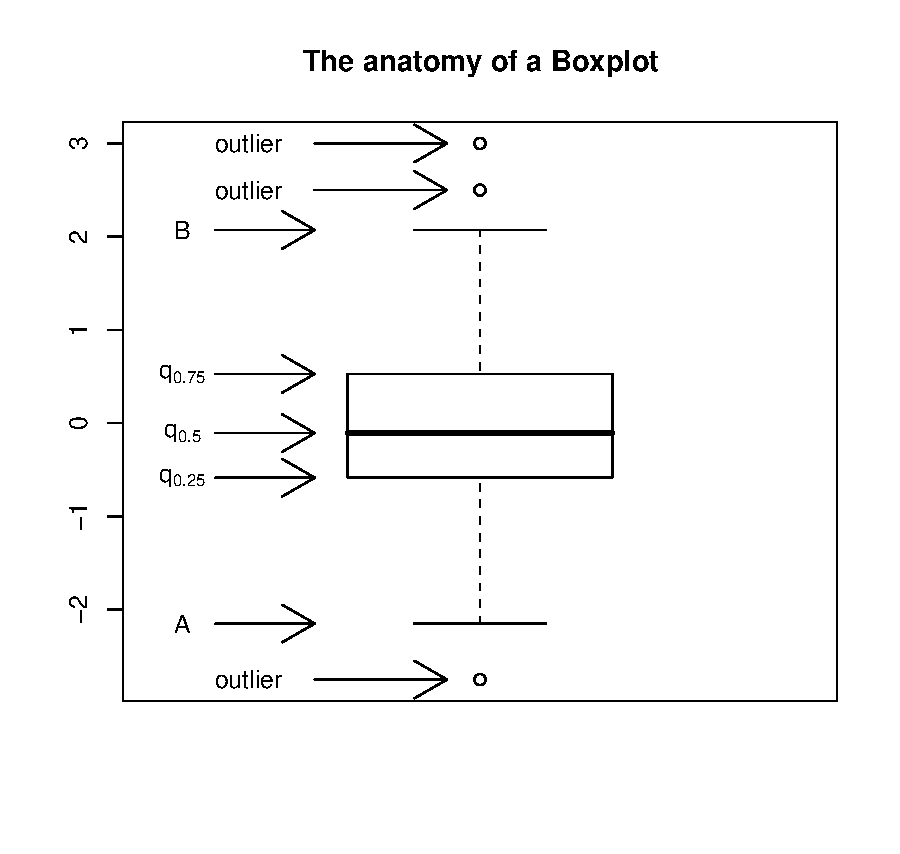
\includegraphics{plots/eda-003}
\end{frame}

\end{document}
